\documentclass{article}
\usepackage{amssymb,amsfonts,amsmath,mathrsfs}
\usepackage[pdftex]{graphicx}
\usepackage{caption}
\usepackage[skip=0cm,list=true,labelfont=it]{subcaption}
\usepackage[top=2cm, bottom=2.2cm, right=2cm, left=2cm]{geometry}
\bibliographystyle{unsrt}
\usepackage{color}
\usepackage{braket}
\usepackage{sectsty}
\usepackage{fancyhdr}
\usepackage{tipa}
\usepackage{setspace}
\usepackage{hyperref}
\usepackage{wrapfig}
\usepackage{graphicx}
\usepackage[export]{adjustbox}
\hypersetup{
    colorlinks=true,
    linkcolor=blue,
    filecolor=magenta,      
    urlcolor=blue,
    citecolor=black
}
\newcommand{\lambdabar}{\mbox{\textipa{\textcrlambda}}}

%\usepackage[numbers,sort&compress]{natbib}

\sectionfont{\fontsize{10}{10}\selectfont}
\subsectionfont{\fontsize{10}{10}\selectfont}
 
\pagestyle{plain}
\begin{document}

\section{Pipeline for generating diffuse scattering maps from experimental data}

While automated programs have been developed to reconstruct reciprocal space maps from Bragg diffraction data, there is minimal software that can process diffuse scattering data. Further, there are no established programs for modeling the diffuse signal. We aimed to develop a pipeline for generating three-dimensional diffuse scattering maps from experimental data that could be easily tuned to both accommodate various data collection choices and fit the evolving needs of downstream analysis. Thus, we emphasize flexibility and convenience rather than speed. This repository contains the result of that endeavor. User choices include degree of map oversampling relative to integral Miller indices and background subtraction strategies, and the scripts have been coded in Python for ease of use and adaptation. Currently only data collected by the rotation method are supported, but we hope in future iterations to enable processing of serial data. Please direct any questions and feedback to \url{apeck@stanford.edu}.

\subsection{Workflow of map construction}
\begin{figure}[htb!]
\centering
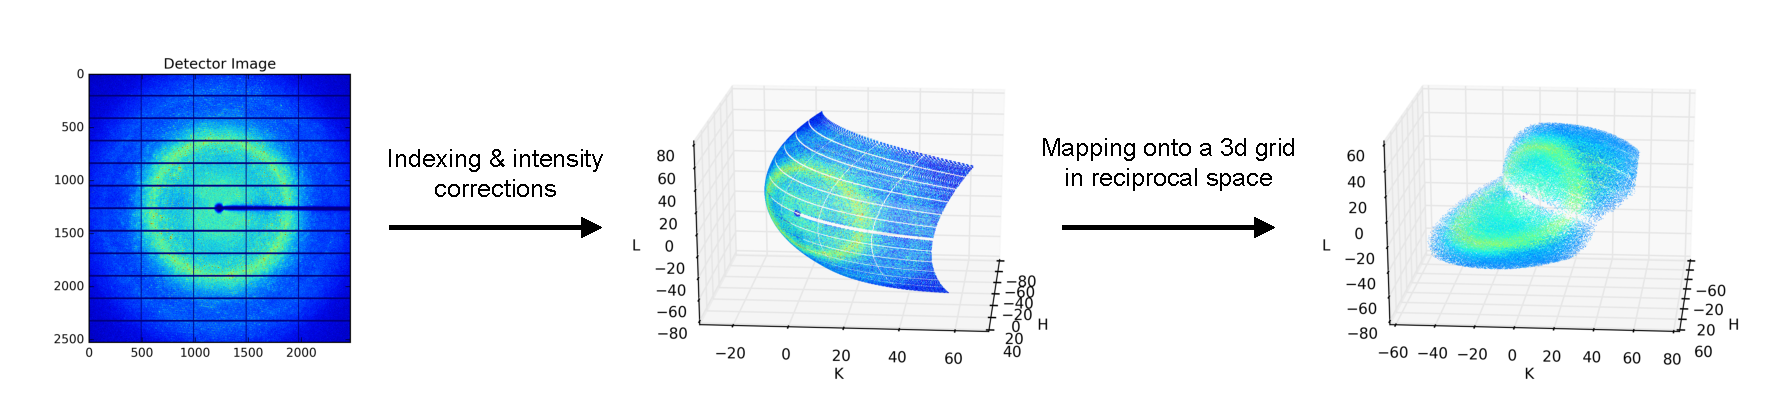
\includegraphics[width=1.0\textwidth]{figures/workflow.pdf}
\caption{\textbf{Schematic of procedure for generating 3d diffuse scattering maps from diffraction images.} }
\end{figure}
\begin{itemize}
%
\item \emph{Step 0: Indexing Bragg reflections by XDS.} 
Downstream steps use batch-refined parameters from XDS \cite{xds}.
%
\item \emph{Step 1: Generation of systems file.} 
The following command extracts information from the XDS output files and stores them in a reference dictionary, named system.pickle:
\\[0.2cm]
\texttt{ \detokenize{ $ python generate_system.py [XDS directory] [map directory] [image type]}}
\\[0.2cm]
Full paths to the XDS output and map building directories must be provided. Currently supported image types are .npy, .h5, and .img; the \texttt{\detokenize{cbf_to_npy.py}} script (following the example of DIALS \cite{dials}) can convert cbf to numpy format. The user will be prompted for which corrections to apply. In the absence of XDS files (e.g. for synthetic data), the system.pickle file can be generated manually.
%
\item \emph{Step 2: Indexing all pixels.} 
All pixels in the dataset are indexed using parameters from system.pickle. Additionally, geometrical distortions are accounted for and per-image scale factors are applied at this stage. Usage:
\\[0.2cm]
\texttt{ \$ python index.py [map directory] [image directory]}
\\[0.2cm]
Output is a numpy array per image of shape (n\_pixels, 4), with columns (h,k,l,I). Correct indexing is checked by computing the residual with the pixel coordinates/Bragg positions determined by XDS, if available.
%
\item \emph{Step 3: Providing map specifications.}
The following command prompts the user for the desired final resolution and degree of oversampling relative to the Miller indices for the final map:
\\[0.2cm]
\texttt{\detokenize{$ python amend_system.py system.pickle}}
%
\item \emph{Step 4: Masking Bragg peaks.} 
Bragg peaks are masked in a series of steps. The first step is parallelized over the number of batches of images in the dataset (determined by XDS), and for each batch predicts the extent of Bragg peaks whose centers lie in the oscillation range spanned by that batch:
\\[0.2cm]
\texttt{\detokenize{ $ python mask_bragg.py generate system.pickle [sigma_n] [absences] [batch number]}}
\\[0.2cm]
Here, the \texttt{\detokenize{sigma_n}} parameter tunes the dimensions of integration region around the center of the Bragg peak; recommended values are 3-5 \cite{pmid20124693}. The \texttt{\detokenize{absences}} input determines whether systematic absences are accounted for: e.g. `000' for none, and `222' for a 2-fold screw axis along each lattice direction. Running this command generates a dictionary whose keys specify the pixels that either coincide with or are predicted to be spanned by a Bragg peak. The output from each batch can be compiled into a single file with the following command: 
\\[0.2cm]
\texttt{ \detokenize{$ python mask_bragg.py compile system.pickle}}
\\[0.2cm]
This information can then be used to remove the Bragg signal with the following command:
\\[0.2cm]
\texttt{ \detokenize{$ python mask_bragg.py apply system.pickle [bragg sigma] [outlier sigma]}}
\\[0.2cm]
where the parameters \texttt{ \detokenize{bragg sigma}} and \texttt{ \detokenize{outlier sigma}} set the thresholds at which pixels are considered outliers and masked. This procedure is explained in more detail below. Output is stored in the directory \texttt{ \detokenize{maskedI}}. Complete removal of the Bragg signal can be checked by the following command:
\\[0.2cm]
\texttt{ \detokenize{$ python check_masks.py} system.pickle}
\\[0.2cm]
which plots the radial pixel intensity distributions before and after removal of the Bragg signal.
%
\item \emph{Step 5: Elimination of parasitic scattering.} 
The command below is not a necessary step, but recommended to check that the overall measured intensity across the rotation range remains roughly constant:
\\[0.2cm]
\texttt{ \detokenize{$ python eliminate_parasitic.py profile system.pickle [hklI directory] [number of bins]}}
\\[0.2cm]
Inputs are the directory that contains the processed intensities (generally \texttt{\detokenize{maskedI}}) and the number of bins across which to compute the radial intensity profile for each image. Outputs are a matrix (\texttt{\detokenize{rI_matrix}}) and plots of the radial intensity profiles, saved to \texttt{\detokenize{temp}} and  \texttt{\detokenize{checks}} folders within the map processing directory. If there is significant variance between the radial intensity profiles across the rotation range, e.g. due to parasitic scattering, then elimination of this signal can be performed by modifying \texttt{ \detokenize{eliminate_parasitic.py}} to specify a background removal strategy and running the following command:
\\[0.2cm]
\texttt{ \detokenize{$ python eliminate_parasitic.py remove system.pickle [hklI directory] [rI_matrix]}}
\\[0.2cm]
Strategies available to remove parasitic scattering are discussed in more detail below. The first command in this step can then be re-run with the directory name of the processed intensities, \texttt{\detokenize{processedI}}, to check the adequacy of the background removal strategy.
%
\item \emph{Step 6: Reconstruction into 3d maps.}
Diffuse scattering maps are constructed as three-dimensional grids in reciprocal space whose nodes oversample Miller indices by the user-decided factor along each lattice direction. Indexed and processed intensities are binned into cubic voxels centered on these nodes, and this procedure is parallelized across a total of \texttt{\detokenize{num_shells}} resolution shells with the following command:
\\[0.2cm]
\texttt{ \detokenize{$ python construct_maps.py compile system.pickle [hklI directory] [num_shells] [nth shell]}}
\\[0.2cm]
The intermediate output is compiled into a single file by averaging the binned intensities to estimate $I(\mathbf{q})$ at the center of each voxel, thereby generating the final three-dimensional map:
\\[0.2cm]
\texttt{ \detokenize{$ python construct_maps.py reduce system.pickle [num_shells]}}
\\[0.2cm]
Outputs are \texttt{ \detokenize{final_maps.h5}} and \texttt{ \detokenize{shell_statistics.h5}}, dictionaries that respectively contain 3d maps and the median by resolution shell of the intensities, signal-to-noise ratio (estimated as $\langle I \rangle / \sigma(\langle I \rangle)$ of each voxel), and the number of pixels per voxel.
%
\item \emph{Step 7: Map post-processing.}
To prepare the maps for downstream analysis, symmetrization and subtraction of the radial average can be performed with:
\\[0.2cm]
\texttt{ \detokenize{$ python map_statistics.py system.pickle [point_group] final_maps.h5 [n_bins] [output_path]}}
\\[0.2cm]
This script can be found in the \texttt{models} directory. In the given output path, it saves \texttt{ \detokenize{processed_maps.h5}}, a dictionary that contains the original map, the map symmetrized by averaging Laue- and Friedel-equivalent voxels, the symmetrized map after subtracting the average radial intensity, and a map of the voxel multiplicities. Also saved is \texttt{\detokenize{symm_statistics.pickle}}, which computes the correlation coefficient between 1. voxels related by Friedel symmetry, 2. the original and Friedel-symmetrized maps, and 3. the original and Laue-symmetrized maps across \texttt{\detokenize{n_bins}} resolution shells.
\end{itemize}


\subsubsection{Corrections for geometrical distortions}
The following corrections are supported:
\begin{enumerate}
%
\item Solid angle normalization, which corrects for the fact that measured intensities are proportional to the solid angle subtended by each pixel. As intensities of the final maps are not on an absolute scale, here we correct for the relative rather than absolute solid angle subtended by each pixel, which is proportional to $\cos^3{\theta}$, where $\theta$ is the angle between the incident and scattered beams \cite{wall2009}.
%
\item Polarization correction, which accounts for the polarization of the x-ray beam. The correction factor, given below, is calculated as implemented in Thor \cite{thor} and described in Ref. \cite{hura2000}:
\begin{equation}
P_c = P_f ( 1 - \sin^2{\phi} \sin^2{2\theta} ) + (1-P_f) ( 1 - \cos^2{\phi} \sin^2{2\theta} )
\end{equation}
where $P_f$ is the fraction of polarization of the x-ray beam, $\phi$ is an angle (aligned with the $y$-axis) in the plane of the detector, and $2\theta$ is the diffraction angle.
%
\item Parallax correction, which accounts for the shift in position between where photons are detected and recorded, resulting from the absorption properties and thickness of silicon detectors. The correction is small, but has been recommended for data collected on Pilatus detectors. Here we follow the implementation used in DIALS: \url{https://github.com/cctbx/cctbx_project/blob/b0460954eac07a3a3639dbe7efd942c21e12ebc1/dxtbx/model/parallax_correction.h}
%
\end{enumerate}
%
Note that Lorentz corrections are unnecessary, as pixel intensities are averaged rather than integrated, and diffuse features tend to extend across large regions of reciprocal space, in which case the Lorentz factor is to a first approximation independent of scattering angle \cite{boysen1987}.

\subsubsection{Masking of Bragg peaks}

Here we implement a two-pronged approach to eliminate the Bragg signal. The first step uses the algorithm described in Ref. \cite{pmid20124693} to predict pixels that will be spanned by Bragg peaks based on the crystal and detector geometries. These pixels are subsequently masked if their intensities exceed three standard deviations above the mean intensity of neighboring, unmarked pixels in a 30 x 30 pixel window centered on the Bragg reflection. The second step removes pixels whose intensities exceed the median radial intensity by more than five times the median absolute deviation of the resolution shell in question. Together, these steps ensure the complete removal of the Bragg signal (including from oddly-shaped peaks that elude the spot prediction algorithm) and eliminate other high intensity contaminants (e.g. from the mount). The window size and thresholds noted here are settings that we empirically found to work well for three different datasets, but these are readily adjusted by the user. Another tunable parameter is $\sigma_n$, which controls the threshold at which pixels are considered too distant from the center of a Bragg peak to likely be spanned by that reflection, as shown below.

\begin{figure}[htb!]
\centering
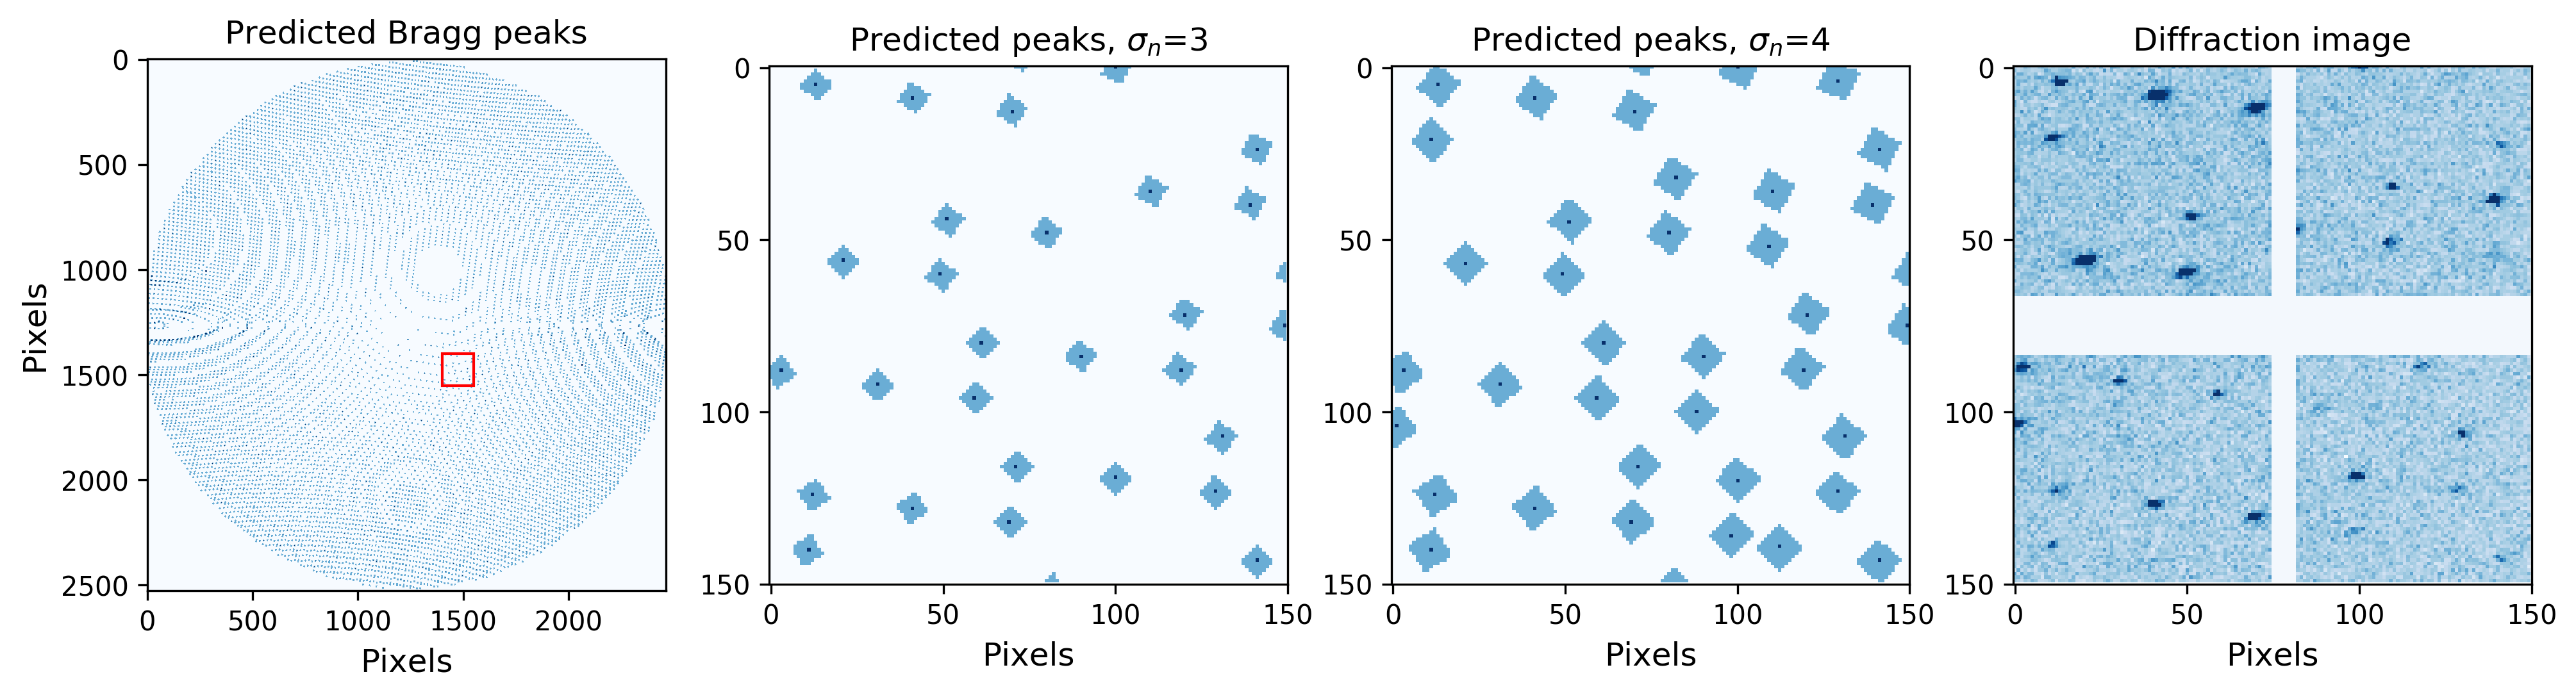
\includegraphics[width=0.9\textwidth]{figures/bragg_masks.png}
\caption{\textbf{Bragg peak shape prediction.} Example output from our implementation of the spot prediction algorithm described in Ref. \cite{pmid20124693}. The $\sigma_n$ parameter tunes how far out (both in detector and rotation space) Bragg peaks are predicted to extend. In the central panels, blue marks pixels predicted to be spanned by a Bragg reflection. }\label{bragg_masks}
\end{figure}

\subsubsection{Elimination of parasitic scattering and other intensity corrections}

In addition to the above corrections, untrusted regions of the detector (as defined in the XDS.INP file) are ignored, and per-image scale factors computed by XDS are applied \cite{pmid20124693}. Though the latter corrects for much of the variation in overall measured intensity across the rotation range, the following additional strategies to eliminate confounding sources of variance (unrelated to the macromolecular diffuse signal) are available:
\begin{enumerate}
%
\item Subtraction of a scaled paratone scattering profile from each image; we anticipate this to be useful for crystals coated in oil to prevent dehydration during data collection. The scale factor is determined on an image-by-image basis by fitting the paratone scattering profile to the image's radial profile between $\mathbf{s}$ = 0.1 and $\mathbf{s}$ = 0.3 \AA{}, where paratone scattering shows a peak.
%
\item Subtraction of scaled paratone or water scattering profiles from each image by minimizing the pairwise difference between all images' radial profiles. The scattering profiles are sourced from nonBragg (\url{http://bl831.als.lbl.gov/~jamesh/nonBragg/}), where the structure factors for other likely sources of radially symmetric scattering are also available.
%
\item Principal component analysis, which identifies variance in the radial intensity profiles of the processed diffraction images. The user can choose how many of the top (largest eigenvalue) principal components to use for removing this variance.
%
\end{enumerate}
%

As an example, the use of these methods to eliminate parasitic scattering from paratone is shown below for a diffraction dataset of cyclophilin A \cite{sbdb68}.

\begin{figure}[htb!]
\centering
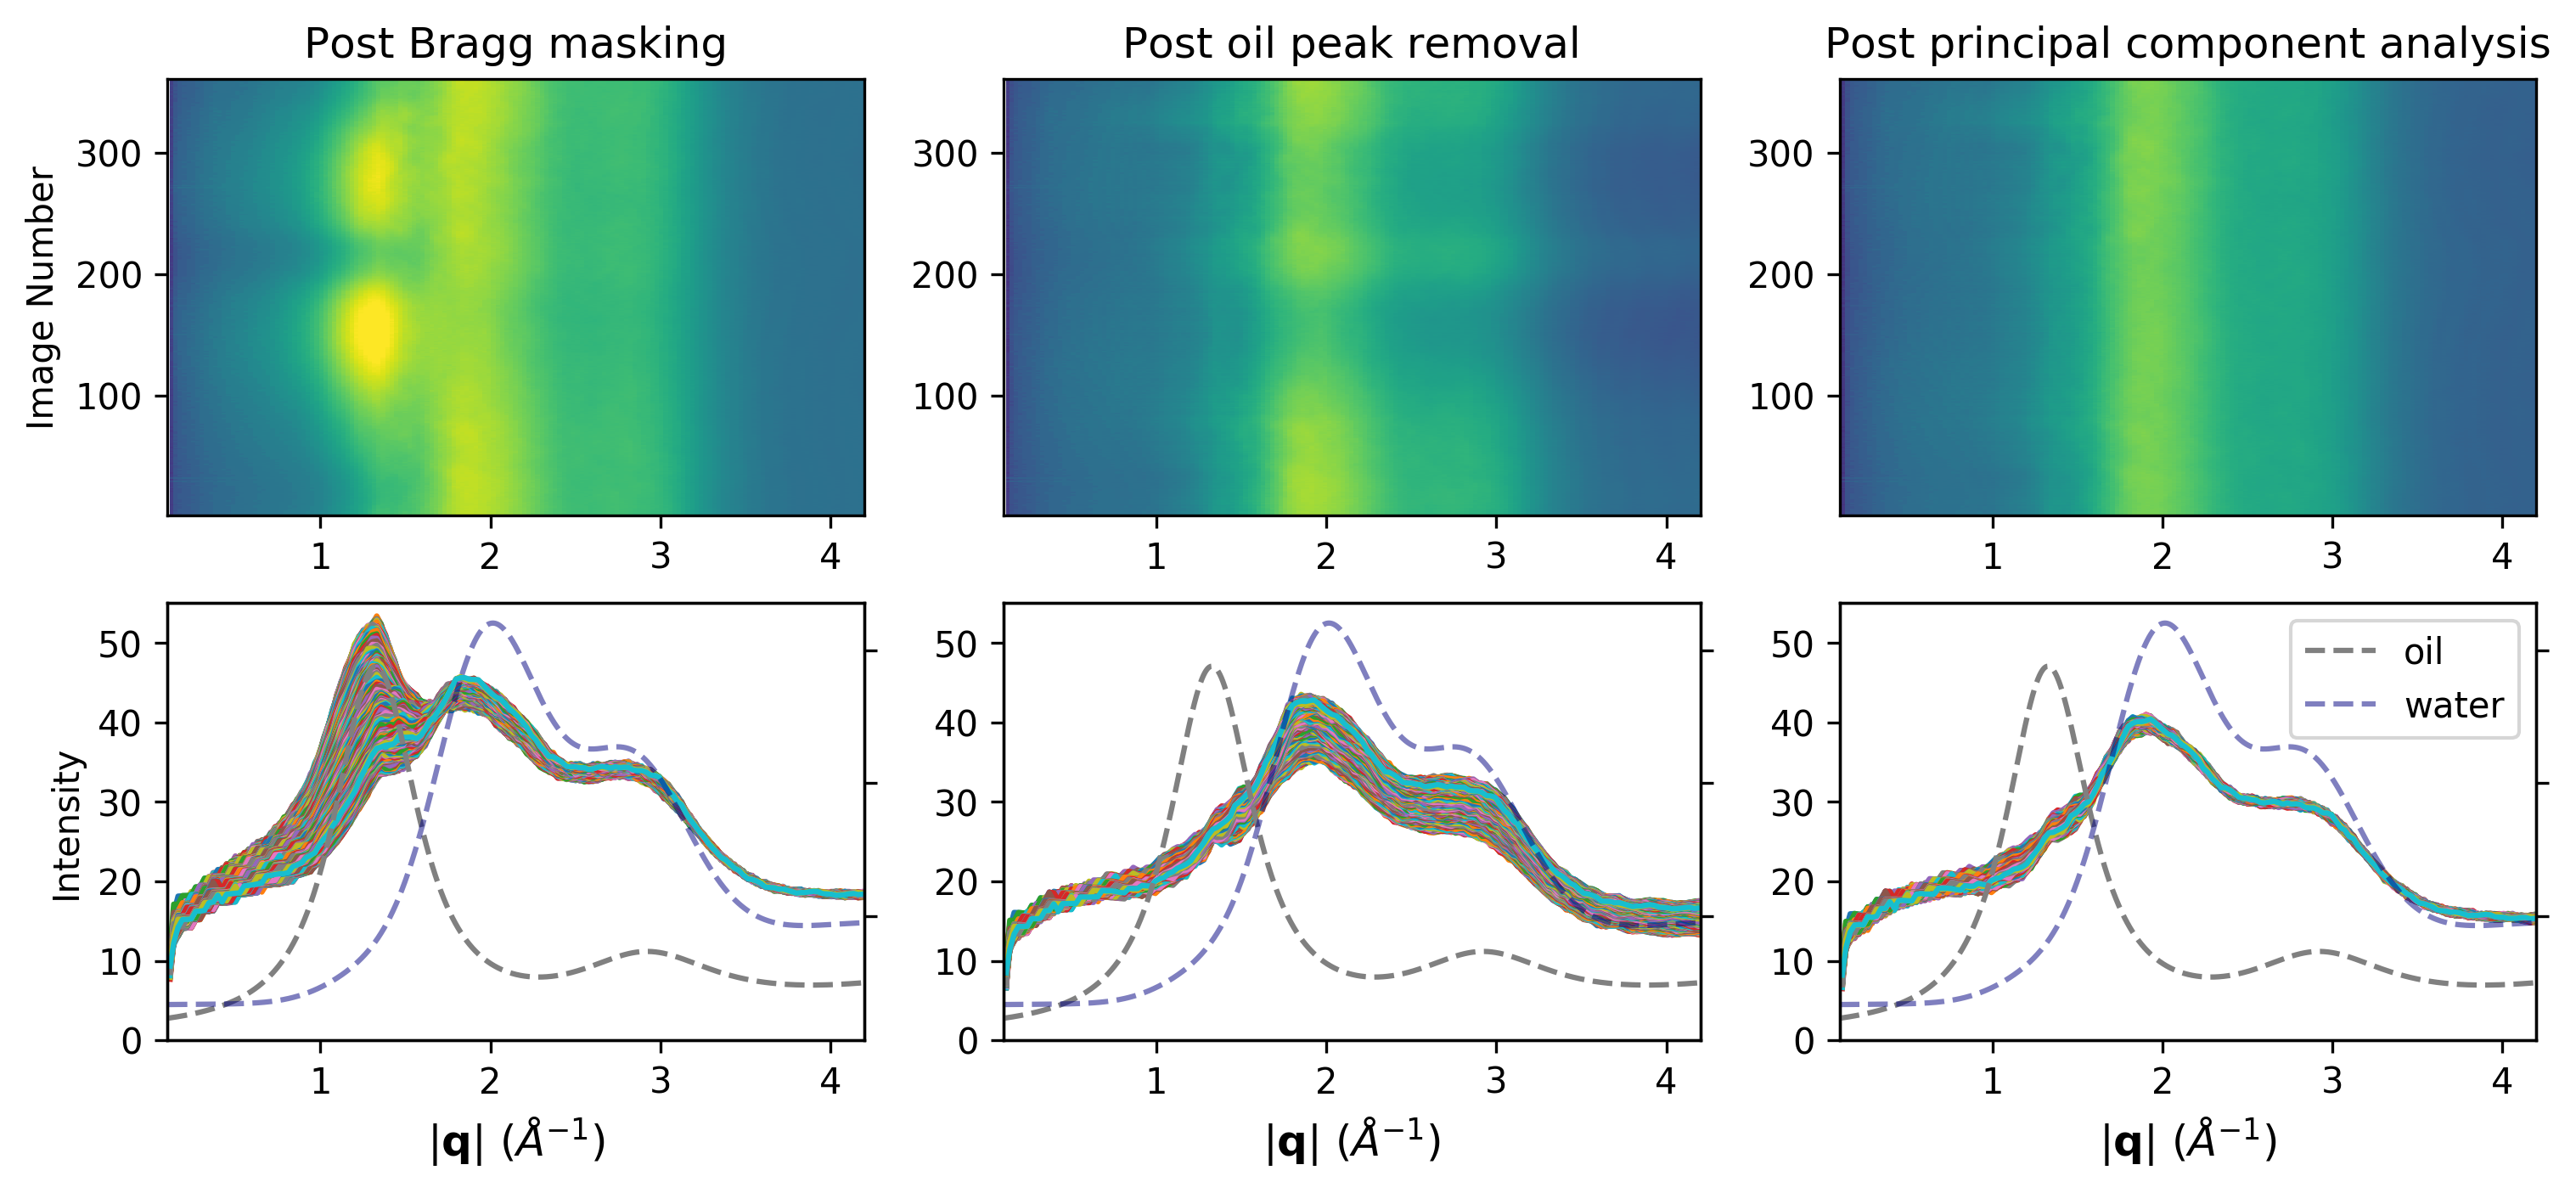
\includegraphics[width=0.8\textwidth]{figures/parasitic.png}
\caption{\textbf{Example approach for eliminating parasitic scattering from paratone.} A radially symmetric peak at $ \vert \mathbf{q} \vert $ = 1.3 \AA{} was variably observed in the radial intensity profiles of the intensities of the cyclophilin A dataset after removal of the Bragg signal (left panels). This was consistent with parasitic scattering from paratone oil and removed by subtraction of a scaled paratone profile (center) panels, followed by removal of residual variance by principal component analysis (right panels). }\label{parasitic}
\end{figure}

\subsubsection{Validation of approach}

The above strategy was evaluated by generating a synthetic dataset of the symmetrized molecular transform of cyclophilin A using the Thor software package \cite{thor}. The dataset consisted of 360 images, each separated by 0.5$^{\circ}$, simulating scattering on a Pilatus detector (albeit without geometrical distortions; also note that this synthetic dataset does not test the Bragg peak masking procedure). A comparison of the reconstruction procedure from the simulated rotation data versus direct calculation of $I(\mathbf{q})$ is shown below. Also shown is an example of the standard output of the indexing step, which checks the accuracy of the indexing implemented here by comparison to the XDS-calculated coordinates if the latter are available.

\begin{figure}[htb!]
\centering
\begin{subfigure}[t]{0.02\textwidth}
\textbf{A}
\end{subfigure}
\begin{subfigure}[t]{0.45\textwidth}
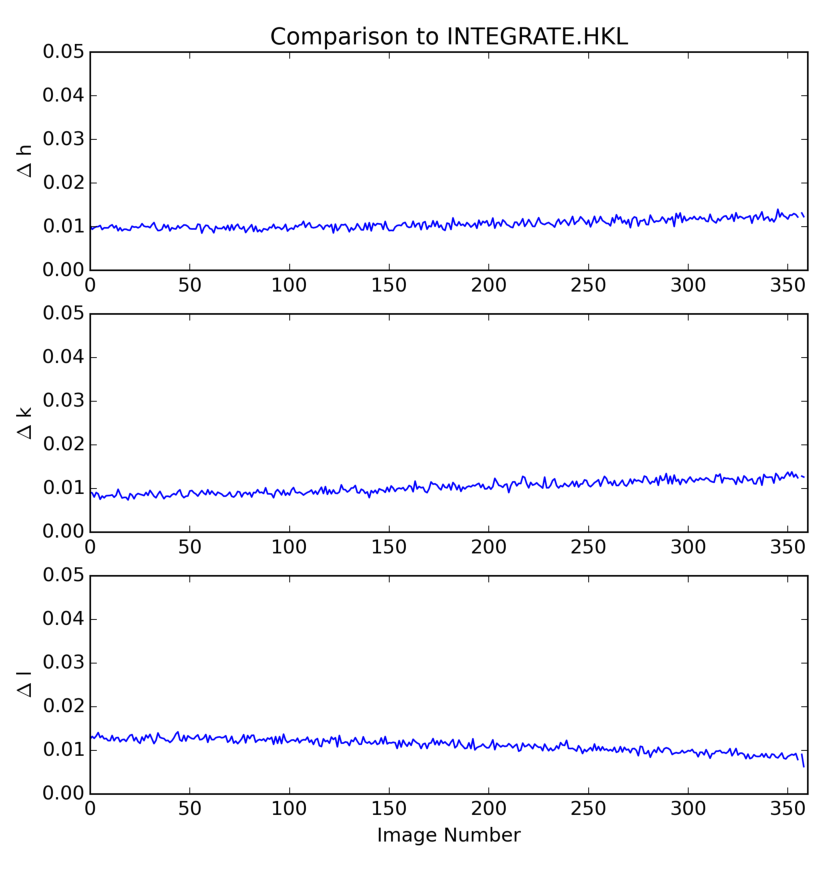
\includegraphics[width=\textwidth,valign=t]{figures/validation1}
\end{subfigure}
\begin{subfigure}[t]{0.02\textwidth}
\textbf{B}
\end{subfigure}
\begin{subfigure}[t]{0.45\textwidth}
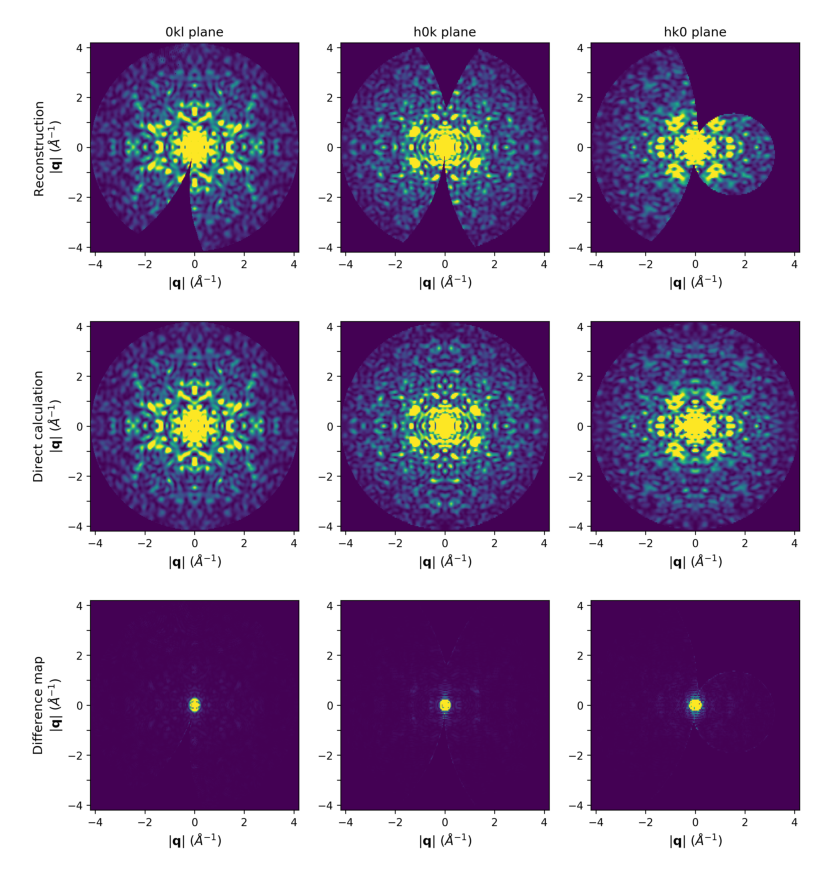
\includegraphics[width=\textwidth,valign=t]{figures/validation2}
\end{subfigure}
\caption{\textbf{Validation of map construction procedure.} (A) Example plot showing the residual between the reciprocal space coordinates computed by our indexing script and XDS. (B) Comparison of the reconstruction procedure outlined above for a synthetic dataset versus direct calculation of $I(\mathbf{q})$ for a 3x-oversampled reciprocal space map. Although the reconstruction underestimates the intensity of voxels at very low resolution, this error is not expected to be pronounced for experimental diffuse scattering maps, in which $I(\mathbf{q})$ at low resolution is not pronounced but rather damped by disorder. }\label{validation}
\end{figure}

\newpage
\bibliography{instructions}

\end{document}